\onehalfspacing
\section{Đề số 23}
\graphicspath{{./img/}}
\begin{bt} 
    Thực hiện phép tính:
   \begin{enumerate}[a.]
    \item $A=\frac{155-\frac{10}{7}-\frac{5}{11}+\frac{5}{23}}{403-\frac{26}{7}-\frac{13}{11}+\frac{13}{23}}+\frac{\frac{3}{5}+\frac{3}{13}-0,9}{\frac{7}{91}+0,2-\frac{3}{10}}$
    \item $B=\frac{2^{12} \cdot 3^5-4^6 \cdot 9^2}{\left(2^2 \cdot 3\right)^6+8^4 \cdot 3^5}+\frac{5^{10} \cdot 7^3-25^5 \cdot 49^2}{(125 \cdot 7)^3+5^9 \cdot 14^3}$
   \end{enumerate}
\loigiai{
    \begin{enumerate}
        \item $ A=\frac{155-\frac{10}{7}-\frac{5}{11}+\frac{5}{23}}{403-\frac{26}{7}-\frac{13}{11}+\frac{13}{23}}+\frac{\frac{3}{5}+\frac{3}{13}-0,9}{\frac{7}{91}+0,2-\frac{3}{10}}=\frac{5\left(31-\frac{2}{7}-\frac{1}{11}+\frac{1}{23}\right)}{13\left(31-\frac{2}{7}-\frac{1}{11}+\frac{1}{23}\right)}+\frac{\frac{3}{5}+\frac{3}{13}-\frac{9}{10}}{\frac{1}{13}+\frac{1}{5}-\frac{3}{10}}$\\[5px] 
        $=\frac{5\left(31-\frac{2}{7}-\frac{1}{11}+\frac{1}{23}\right)}{13\left(31-\frac{2}{7}-\frac{1}{11}+\frac{1}{23}\right)}+\frac{3\left(\frac{1}{5}+\frac{1}{13}-\frac{3}{10}\right)}{\frac{1}{5}+\frac{1}{13}-\frac{3}{10}} \\[5px] =\frac{5}{13}+3=3 \frac{5}{13}$
        \item $B=\frac{2^{12} \cdot 3^5-4^6 \cdot 9^2}{\left(2^2 \cdot 3\right)^6+8^4 \cdot 3^5}-\frac{5^{10} \cdot 7^3-25^5 \cdot 49^2}{(125 \cdot 7)^3+5^9 \cdot 14^3}=\frac{2^{12} \cdot 3^5-2^{12} \cdot 3^4}{2^{12} \cdot 3^6+2^{12} \cdot 3^5}-\frac{5^{10} \cdot 7^3-5^{10} \cdot 7^4}{5^9 \cdot 7^3+5^9 \cdot 7^3 \cdot 2^3} \\[5px] =\frac{2^{12} \cdot 3^4(3-1)}{2^{12} \cdot 3^5(3+1)}-\frac{5^{10} \cdot 7^3(1-7)}{5^9 \cdot 7^3\left(1+2^3\right)} \\[5px] =\frac{2}{3 \cdot 4}-\frac{5 \cdot(-6)}{9}=\frac{1}{6}+\frac{10}{3}=\frac{21}{6}=\frac{7}{2}$
    \end{enumerate}
}
\end{bt}

\begin{bt}
    \hfill
	\begin{enumerate}[a.]
        \item Chứng minh rằng: $3^{n+2}-2^{n+2}+3^n-2^n$ chia hết cho 10 với mọi số nguyên dương $\mathrm{n}$.
        \item Tìm giá trị nhỏ nhất của biểu thức : $A=|2014-x|+|2015-x|+|2016-x|$
        \item Tìm x, y thuộc $\mathrm{Z}$ biết : $25-y^2=8(x-2015)^2$
    \end{enumerate}
	\loigiai{
        \begin{enumerate}
            \item $\text {Ta có }: 3^{n+2}-2^{n+2}+3^n-2^n=3^n \cdot 9-2^n \cdot 4+3^n-2^n \\[5px]
            =3^n \cdot 10-2^n \cdot 5=3^n \cdot 10-2^{n-1} \cdot 10 \\[5px]
            =10\left(3^n-2^{n-1}\right) \vdots 10$\\[5px]
            Vậy $3^{n+2}-2^{n+2}+3^n-2^n$ chia hết cho 10 với mọi số nguyên dương $n$.
            \item Vì $|2015-x| \geq 0$ nên :\\[5px]
            $A=|2014-x|+|2015-x|+|2016-x| \geq|2014-x|+|2016-x|$\\[5px]
            Dấu " $=$ " xảy ra khi và chỉ khi $x=2015(1)$\\[5px]
            Ta có : $|2014-x|+|2016-x|=|x-2014|+|2016-x| \geq|x-2014+2016-x|=2$\\[5px]
            Dấu "=" xảy ra khi và chỉ khi $(x-2014)(2016-x) \geq 0$, suy ra :\\[5px]
            $2014 \leq x \leq 2016(2)$\\[5px]
            Từ (1) và (2) suy ra $\mathrm{A} \geq 2$. Dấu “=" xảy ra khi và chỉ khi $\mathrm{x}=2015$.\\[5px]
            Vậy $\mathrm{A}$ nhỏ nhất bằng 2 khi $x=2015$.
            \item Ta có : $25-y^2 \leq 25 \Rightarrow 8(x-2015)^2 \leq 25 \Rightarrow(x-2015)^2<4$.\\[5px]
            Do $x$ nguyên nên $(x-2015)^2$ là số chính phương. Có 2 trường hợp xảy ra :\\[5px]
            TH $1:(x-2015)^2=0 \Rightarrow x=2015$, khi đó $\mathrm{y}=5$ hoặc $\mathrm{y}=-5$.\\[5px]
            TH $2:(x-2015)^2=1 \Rightarrow\left[\begin{array}{l}x-2015=1 \\[5px] x-2015=-1\end{array} \Rightarrow\left[\begin{array}{l}x=2016 \\[5px] x=2014\end{array}\right.\right.$\\[5px]
            Với $x=2016$ hoặc $x=2014$ thì $y^2=17$ (loại)\\[5px]
            Vậy $x=2015, y=5$ và $x=2015, y=-5$
        \end{enumerate}
    } 
\end{bt}

\begin{bt}
    \hfill
    \begin{enumerate}[a.]
        \item Cho $\frac{x+16}{9}=\frac{y-25}{-16}=\frac{z+49}{25}$ và $4 x^3-3=29$. Tính: $\mathrm{x}-2 \mathrm{y}+3 \mathrm{z}$
        \item Cho $f(x)=\mathrm{ax}^3+4 x\left(x^2-1\right)+8$ và $g(x)=\mathrm{x}^3+4 x(b x+1)+c-3$ trong đó $\mathrm{a}, \mathrm{b}$, $c$ là hằng số. 
        
        Xác định $a, b, c$ để $f(x)=g(x)$.
    \end{enumerate}
	\loigiai{
        \begin{enumerate}
            \item Ta có : $4 x^3-3=29 \Rightarrow 4 x^3=32 \Rightarrow x^3=8 \Rightarrow x=2$.\\[5px]
            Thay vào tỷ lệ thức ta được :\\[5px] 
            $\frac{2+16}{9}=\frac{y-25}{-16}=\frac{z+49}{25} \Rightarrow \frac{y-25}{-16}=\frac{z+49}{25}=2$\\[5px]
            $\Rightarrow y=-7, z=1$\\[5px]
            Vậy $x-2 y+3 z=2-2 \cdot(-7)+3.1=19$
            \item Ta có : $\mathrm{f}(\mathrm{x})=\mathrm{ax}^3+4 x\left(x^2-1\right)+8=\mathrm{ax}^3+4 x^3-4 x+8=(a+4) x^3-4 x+8$\\[5px]
            $\mathrm{g}(\mathrm{x})=\mathrm{x}^3-4 x(b x+1)+c-3=\mathrm{x}^3-4 b x^2-4 x+c-3$\\[5px]
            Do $\mathrm{f}(\mathrm{x})=\mathrm{g}(\mathrm{x})$ nên chọn $\mathrm{x}$ bằng $0 ; 1 ;-1$ ta được:\\[5px]
            $\mathrm{f}(0)=\mathrm{g}(0) \Rightarrow 8=\mathrm{c}-3 \Rightarrow \mathrm{c}=11 \Rightarrow g(x)=\mathrm{x}^3-4 b x^2-4 x+8 \\[5px]
            \mathrm{f}(1)=\mathrm{g}(1) \Rightarrow \mathrm{a}+4-4+8=1-4 \mathrm{~b}-4+8 \Rightarrow \mathrm{a}+4 \mathrm{~b}=-3(1) \\[5px]
            \mathrm{f}(-1)=\mathrm{g}(-1) \Rightarrow-\mathrm{a}-4+4+8=-1-4 \mathrm{~b}+4+8 \Rightarrow-\mathrm{a}+4 \mathrm{~b}=3(2)$\\[5px]
            Từ (1) và (2) suy ra: $b=0 ; a=-3$.\\[5px]
            Vậy $a=-3, b=0 ; c=11$\\[5px]
        \end{enumerate}
    }
\end{bt}

\begin{bt}
    Cho tam giác $\mathrm{ABC}$ có $(\mathrm{AB}<\mathrm{AC})$. Gọi $\mathrm{M}$ là trung điểm của $\mathrm{BC}$. Từ $\mathrm{M}$ kẻ đường thẳng vuông góc với tia phân giác của góc $\mathrm{BAC}$ tại $\mathrm{N}$, cắt tia $\mathrm{AB}$ tại $\mathrm{E}$ và cắt tia $\mathrm{AC}$ tại $F$. Chứng minh rằng :
    \begin{enumerate}[a.]
        \item $\mathrm{BE}=\mathrm{CF}$
        \item $A E=\frac{A B+A C}{2}$
    \end{enumerate}
\loigiai{
    $$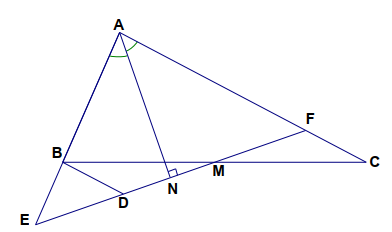
\includegraphics[width=0.45\textwidth]{23-4-lg.png}$$
    \begin{enumerate}
        \item Qua $\mathrm{B}$ kẻ đường thẳng song song với $\mathrm{AC}$, cắt $\mathrm{EF}$ tại $\mathrm{D}$.\\[5px]
        Xét $\triangle \mathrm{MBD}$ và $\triangle \mathrm{MCF}$ có : $D B M=F C M$ (so le trong)\\[5px]
        $\mathrm{MB}=\mathrm{MC} \text { (giả thiết); } B M D=C M F \text { (đối đỉnh) }$\\[5px]
        Do đó: $\triangle \mathrm{MBD}=\triangle \mathrm{MCF}$ (c.g.c) suy ra $\mathrm{BD}=\mathrm{CF}(1)$\\[5px]
        Mặt khác : $\triangle \mathrm{AEF}$ có $\mathrm{AN}$ vừa là đường cao, vừa là đường phân giác nên cân tại $\mathrm{A}$, suy ra $E=M F A$. Mà $B D E=M F A$ (đồng vị) nên $B D E=E$\\[5px]
        Do đó: $\triangle \mathrm{BDE}$ cân tại $\mathrm{B}$, suy ra $\mathrm{BD}=\mathrm{BE}(2)$.\\[5px]
        Từ (1) và (2) suy ra : $B E=C F(\text{đpcm})$
        \item Tam giác $\mathrm{AEF}$ cân tại $\mathrm{A}$ suy ra $\mathrm{AE}=\mathrm{AF}$\\[5px]
        Ta có: $2 \mathrm{AE}=\mathrm{AE}+\mathrm{AF}=(\mathrm{AB}+\mathrm{BD})+(\mathrm{AC}-\mathrm{CF})$\\[5px]
        $=(\mathrm{AB}+\mathrm{AC})+(\mathrm{BD}-\mathrm{CF})=\mathrm{AB}+\mathrm{AC}(\text { do } \mathrm{BE}=\mathrm{CF})$\\[5px]
        Vậy $A E=\frac{A B+A C}{2}$ (đpcm)
    \end{enumerate}
}
\end{bt}

\begin{bt}
   Cho tam giác $\mathrm{ABC}$ có góc $\mathrm{B}$ bằng $45^{\circ}$, góc $\mathrm{C}$ bằng $120^{\circ}$. Trên tia đối của tia $CB$ lấy điểm $\mathrm{D}$ sao cho $\mathrm{CD}=2 \mathrm{CB}$. Tính góc $\mathrm{ADB}$.
\loigiai{
    $$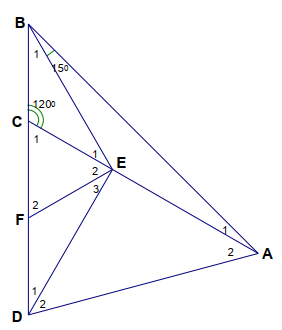
\includegraphics[width=0.4\textwidth]{23-5-lg.png}$$
    Trên CA lấy điểm E sao cho $E B A=15^{\circ} \Rightarrow B_1=30^{\circ}$\\[5px]
    Ta có : $E_1=A_1+E B A=30^{\circ}$, do đó $\triangle \mathrm{CBE}$ cân tại $\mathrm{C} \Rightarrow \mathrm{CB}=\mathrm{CE}$\\[5px]
    Gọi $\mathrm{F}$ là trung điểm $\mathrm{CD} \Rightarrow \mathrm{CB}=\mathrm{CE}=\mathrm{CF}=\mathrm{FD}$\\[5px]
    Tam giác CEF cân tại $C$, lại có $C_1=180^{\circ}-B C A=60^{\circ}$ nên là tam giác đều.\\[5px]
    Như vậy : $\mathrm{CB}=\mathrm{CE}=\mathrm{CF}=\mathrm{FD}=\mathrm{EF}$.\\[5px]
    Suy ra $D_1=E_3$ mà $D_1+E_3=F_2=60^{\circ}\left(\Delta \mathrm{CEF}\right.$ đều) $\Rightarrow D_1=30^{\circ}$\\[5px]
    Xét tam giác $C D E$ ta có: $\quad C E D=180^{\circ}-\left(C_1+D_1\right)=90^{\circ}(1)$\\[5px]
    Ta có : $D_1=B_1 \Rightarrow \mathrm{EB}=\mathrm{ED}, A_1=E B A \Rightarrow \mathrm{EA}=\mathrm{EB} \Rightarrow \mathrm{ED}=\mathrm{ED}$\\[5px]
    Từ (1) và $(2) \Rightarrow$ Tam giác $E D A$ vuông cân tại $\mathrm{E} \Rightarrow D_2=45^{\circ}$\\[5px]
    Vậy $A D B=D_1+D_2=30^{\circ}+45^{\circ}=75^{\circ}$
}
\end{bt}

